\documentclass{article} 
\usepackage{polski} %moze wymagac dokonfigurowania latexa, ale jest lepszy niż standardowy babel'owy [polish] 
\usepackage[utf8]{inputenc} 
\usepackage[OT4]{fontenc} 
\usepackage{graphicx,color} %include pdf's (and png's for raster graphics... avoid raster graphics!) 
\usepackage{url} 
\usepackage[pdftex,hyperfootnotes=false,pdfborder={0 0 0}]{hyperref} %za wszystkimi pakietami; pdfborder nie wszedzie tak samo zaimplementowane bo specyfikacja nieprecyzyjna; pod miktex'em po prostu nie widac wtedy ramek


% Zmiana rozmiarów strony tekstu
\addtolength{\voffset}{-1cm}
\addtolength{\hoffset}{-1cm}
\addtolength{\textwidth}{2cm}
\addtolength{\textheight}{2cm}

%bardziej zyciowe parametry sterujace rozmieszczeniem rysunkow
\renewcommand{\topfraction}{.85}
\renewcommand{\bottomfraction}{.7}
\renewcommand{\textfraction}{.15}
\renewcommand{\floatpagefraction}{.66}
\renewcommand{\dbltopfraction}{.66}
\renewcommand{\dblfloatpagefraction}{.66}
\setcounter{topnumber}{9}
\setcounter{bottomnumber}{9}
\setcounter{totalnumber}{20}
\setcounter{dbltopnumber}{9}

% własny bullet list z malymi odstepami
\newenvironment{tightlist}{
\begin{itemize}
  \setlength{\itemsep}{1pt}
  \setlength{\parskip}{0pt}
  \setlength{\parsep}{0pt}}
{\end{itemize}}

%obrazkow szukamy w nastepujacym katalogu:
\graphicspath{{pics/}}



%\title{Sprawozdanie z laboratorium:\\Metaheurystyki i Obliczenia Inspirowane Biologicznie}
%\author{}
%\date{}

\begin{document}

\thispagestyle{empty} %bez numeru strony

\begin{center}
{\large{Sprawozdanie z laboratorium:\\
Bioinformatyka\\
(szablon)}}

\vspace{3ex}

Część I: Analiza teoretyczna
%Część II: Algorytmy optymalizacji lokalnej i globalnej, problem QAP
%Część III: Eksperyment: ... (prezentację można zrobić w LaTeX - służy do tego klasa "beamer")

\vspace{3ex}
{\footnotesize\today}

\end{center}


\vspace{10ex}

Prowadzący: prof. dr hab.~inż. Marta Kasprzak

\vspace{5ex}

Autorzy:
\begin{tabular}{lllr}
\textbf{Damian Jurga} & inf..... & I2 & jasiu@serwer.domena.poczta.pl \\
\textbf{Grzegorz Miebs} & inf122453 & I2 & grzegorz.miebs@student.put.poznan.pl \\
\end{tabular}

\vspace{5ex}

Zajęcia środowe, 11:45.

\vspace{35ex}

\noindent Oświadczamy, że niniejsze sprawozdanie zostało przygotowane wyłącznie przez powyższych autorów,
a wszystkie elementy pochodzące z innych źródeł zostały odpowiednio zaznaczone i~są cytowane w bibliografii.  

\newpage



\section{Wstęp}
Celem tego sprawozdania jest przedstawienie teoretycznego opracowania metody heurystycznej rozwiązującej problem sekwencjonowania łańcuchów DNA z błędami pozytywnymi oraz negatywnymi w czasie wielomianowym. Algorytm mając dany na wejściu zbiór oligonukleotydów (tj. ciągów nukleotydów: adeniny, tyminy, guaniny i cytozyny), długość sekwencji oryginalnej, powinien zwrócić jak najdłuższą sekwencję.

W tym celu zaproponowano następujący algorytm: sekwencja jest budowana za pomocą algorytmu wiązkowego, następnie poprawiana algorytmem wspinaczkowym i, jeżeli to możliwe, ponownie przedłużana algorytmem wiązkowym lub poprzez pełny przegląd. Przyjęto szerokość wiązki równą osiem, maksymalną liczbę iteracji algorytmu wspinaczkowego  równą sto oraz granicę długości określającą, czy w trzeciej fazie zostanie zastosowany algorytm wiązkowy, czy pełnego przeglądu równą pięć.
%\section{Implementacja}
\section{Wyniki}

Pomiarów dokonano na %tu uzupełnij dane techniczne komp/proc.
Mierzono czas wykonania, długość sekwencji oraz liczbę wykorzystanych oligonukleotydów.
Wyniki porównano według odległości euklidesowej długości sekwencji wynikowej $n_w$ od długości sekwencji wejściowej $n$:

\begin{equation}
L_2 = \sqrt{(n_w-n)^2} = |n_w-n|
\end{equation}

oraz średniego czasu wykonania.
W obu wypadkach w funkcji długości sekwencji wejściowej i mocy zbioru oligonukleotydów.

\subsection{Wszystkie instancje}

\begin{figure}[h]
\center
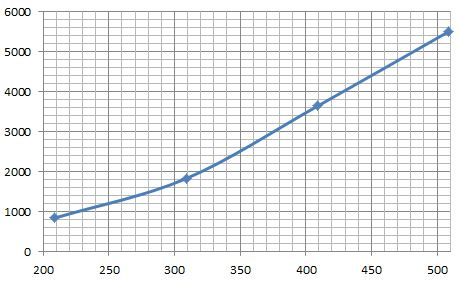
\includegraphics[scale=1]{Przechwytywanie5.jpg}
\caption{\textit{Na osi rzędnych odłożona jest długość sekwencji wejściowej, a na odciętych --- średni czas wykonywania w milisekundach}}
\end{figure}

\begin{figure}[h]
\center
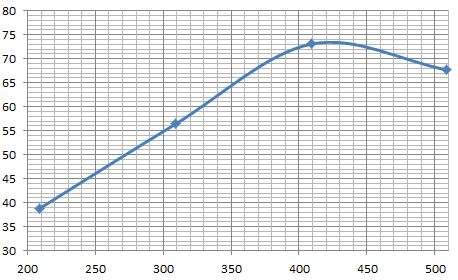
\includegraphics[scale=1]{Przechwytywanie6.jpg}
\caption{\textit{Na osi rzędnych odłożona jest długość sekwencji wejściowej, a na odciętych --- średnia odległość $L_2$}}
\end{figure}

Powyższe wykresy pokazują, że dla zadanego układu instancji testowych średni czas wykonania i średnia odległość $L_2$ jest co najwyżej wielomianem długości sekwencji wejściowej.
Rozważanie wartości w funkcji mocy zbioru nie ma sensu, gdyż w większości przypadków wartość funkcji sprowadzałaby się do wartości funkcji obliczanych dla jednej z typów instancji.

\subsection{Porównanie}

\begin{figure}[h]
\center
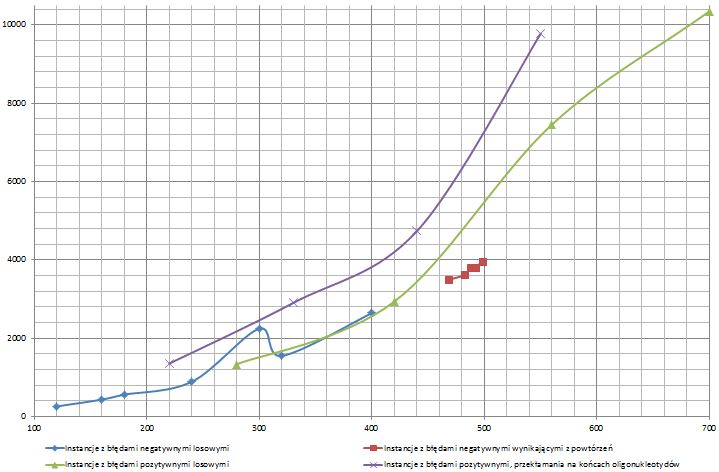
\includegraphics[scale=0.75]{Przechwytywanie.jpg}
\caption{\textit{Na osi rzędnych odłożona jest moc zbioru oligonukleotydów, a na odciętych --- czas wykonywania w milisekundach}}
\end{figure}

\begin{figure}[H]
\makebox[\textwidth][c]{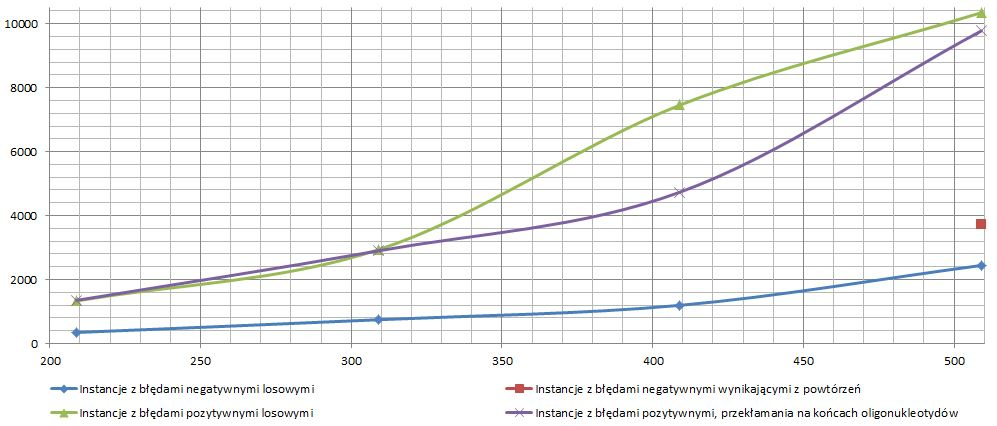
\includegraphics[scale=0.75]{Przechwytywanie4.jpg}}
\caption{\textit{Na osi rzędnych odłożona jest długość sekwencji wejściowej, a na odciętych --- czas wykonywania w milisekundach}}
\end{figure}

Jak widać na rysunkach 3 i 4, najszybciej zbieżne do lokalnego optimum okazały się instancje z błędami negatywnymi, a najwolniej --- z błędami pozytywnymi.
Funkcje czasów wykonania wydają się być ograniczone od góry wielomianami. %trzeciego stopnia?

\begin{figure}[h]
\center
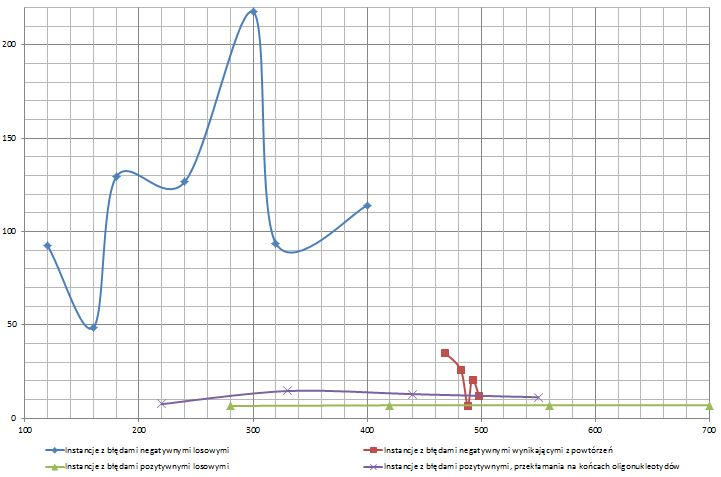
\includegraphics[scale=0.75]{Przechwytywanie3.jpg}
\caption{\textit{Na osi rzędnych odłożona jest moc zbioru oligonukleotydów, a na odciętych --- odległości euklidesowej długości sekwencji wynikowej $n_w$ od długości sekwencji wejściowej $n$}}
\end{figure}

\begin{figure}[h]

\makebox[\textwidth][c]{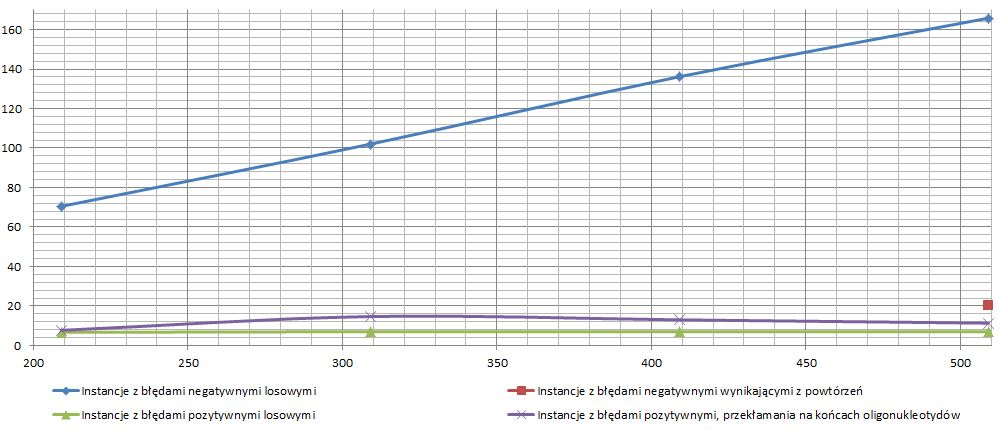
\includegraphics[scale=0.75]{Przechwytywanie2.jpg}}
\caption{\textit{Na osi rzędnych odłożona jest długość sekwencji wejściowej, a na odciętych --- odległości euklidesowej długości sekwencji wynikowej $n_w$ od długości sekwencji wejściowej $n$}}
\end{figure}

Na rysunkach 5 i 6 widać, że instancje z błędami negatywnymi powodowały utworzenie sekwencji wynikowej zdecydowanie bardziej odległej od wejściowej i bardziej zmiennej.
Instancje z błędami pozytywnymi utrzymywały w przybliżeniu stałą odległość $L_2$.

Można zauważyć, że w przypadku instancji z błędami negatywnymi:
\begin{equation}
L_2 \approx 0.31(7)*n+4,08(4)
\end{equation}

\section{Dalsze eksperymenty}

Wyniki sugerują, że dałoby się zaproponować takie parametry algorytmu, by zoptymalizować czas wykonywania i odległość od sekwencji wejściowej.
Jest to problem optymalizacji wielokryterialnej wymagający zbadania wpływu szerokości wiązki, maksymalnej liczby iteracji algorytmu wspinaczkowego, wartości kary oraz granicy długości określającej, czy w trzeciej fazie zostanie zastosowany algorytm wiązkowy, czy pełnego przeglądu, na oba kryteria.

Najprostszym lecz czasochłonnym sposobem wydaje się zastosowanie algorytmu pełnego przeglądu lub wspinaczkowego na charakterystycznych wartościach parametrów wejściowych.
\end{document} 

